%File: formatting-instruction.tex
\documentclass[letterpaper]{article}
\usepackage{graphicx}
\graphicspath{ {Images/} }
\usepackage{aaai}
\usepackage{times}
\usepackage{helvet}
\usepackage{courier}
\frenchspacing
\setlength{\pdfpagewidth}{8.5in}
\setlength{\pdfpageheight}{11in}
\pdfinfo{
/Title {Unsupervised Decomposition of Multi-Author Document}
/Author (Sayantan Sengupta,Kautsya Kanu)}
\setcounter{secnumdepth}{0}  
 \begin{document}
% The file aaai.sty is the style file for AAAI Press 
% proceedings, working notes, and technical reports.
%
\title{Unsupervised Decomposition of Multi-Author \\Document}
\author{Sayantan Sengupta \and   Kautsya Kanu\\ 
Indian Institute of Technology Delhi\\
}
\maketitle
% \begin{abstract}
% \begin{quote}
% AAAI creates proceedings, working notes, and technical reports directly from electronic source furnished by the authors. To ensure that all papers in the publication have a uniform appearance, authors must adhere to the following instructions. 
% \end{quote}
% \end{abstract}
\section{Introduction}
\noindent Here we propose a new unsupervised method for decomposing a multi-author document in to authorial components. We have assumed that we have no prior information about the authors and the documents, except the number of authors of the document. The key idea is to exploit the differences of the grammatical writing styles of the authors and use this information to build paragraph clusters. This is a difficult problem in many levels. It’s easy to decompose based on topics and contexts, which is often known as text segmentation in literature. So it gets difficult to distinguish if multiple authors have written on the same topic. Quantifying the difference of the grammatical writing styles of authors is another big challenge. As there is no prior information/access to the author’s written texts, supervised classification approaches can’t be applied directly. On top of this, the number of author is not known in general of a random a document/article in general (in case of plagiarism). So fixing the number of clusters is another big task. So considering the above constraints, this paper focus more on the feature selection part of the texts which is the most important part of the whole unsupervised clustering, as good features will lead to more precise clustering of the correct sentences to their respective clusters.
The traditional studies on text segmentation, as shown in Choi (2000), Brants et al. (2002), Misra et al. (2009) and Henning and Labor (2009), focus on dividing the the text into significant components such as words, sentences and topics rather than authors. There are almost no approaches, as those in Schaalje et. al. (2013), Segarra et al (2014) and Layton et al. (2013) deal with documents written by a single author only. Koppel et al. (2011) has considered the segmentation of a document according to multi-authorship, this approach requires manual translations and concordance to be available beforehand. Hence their document can only be applied on particular types of documents such as Bible books. Akiva and Koppel (2013) tried to come up with a solution. Their method relies on distance measurement to increase the precision and accuracy of the clustering and classification process. The performance is degraded when the number of authors increases to more than two.


% \begin{itemize}
% \item You must use the latest AAAI Press \LaTeX{} macro.
% \item Download the author kit.
% \item Complete, sign, and return by the deadline the AAAI copyright form (proceedings authors) or distribution license (technical report authors).
% \item Read and format your paper source and PDF according to the formatting instructions for authors.
% \item Submit your electronic files and abstract using our electronic submission form \textbf{on time.}
% \item Submit your copyright form, and any required page or formatting charges to AAAI Press so that they are received by the deadline.
% \item Check every page of your paper before submitting it.
% \end{itemize}

\section{Baseline}
The latest state of the art technique used in this area is described below:
Given a multi-author document written by l authors, it is assumed that every author has written consecutive sentences, and every sentence is completely written by only one of the authors. The approach goes through the following steps:
\begin{itemize}
\item Divide the document into segments of fixed length.
\item Represent the resulted segments as vectors using an appropriate feature set which can differentiate the writing styles among authors (words occurring at least 3 times in the text).
\item Cluster the resulted vectors into l clusters using an appropriate clustering algorithm targeting on high recall rates(GMM with iterative EM algorithm).
\item Re-vectorize the segments using a different feature set to more accurately discriminate the segments in each cluster.
\item Apply the segment Elicitation procedure, which identifies the vital segments from each clusters to improve the precision rates.
\item Re-vectorize all selected segments using another feature set that can capture the differences in the writing styles of all the sentences in a document.
\item Train the classifier using a Naive Bayesian model.
\item Classify each sentence using the learned classifier.
\end{itemize}
\begin{figure}
\caption{•}
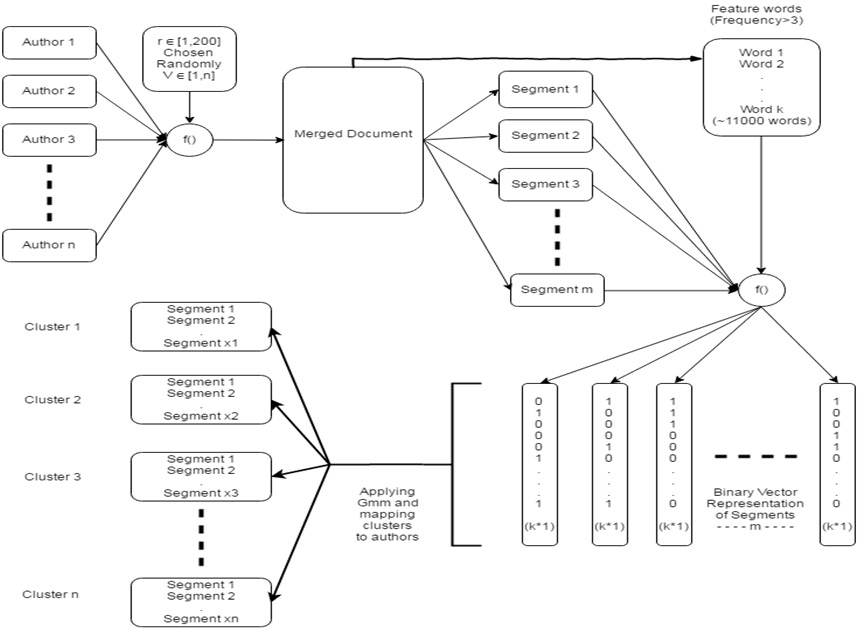
\includegraphics[width=8cm]{u7.jpg}
\centering
\end{figure}
\begin{figure}
\caption{•}
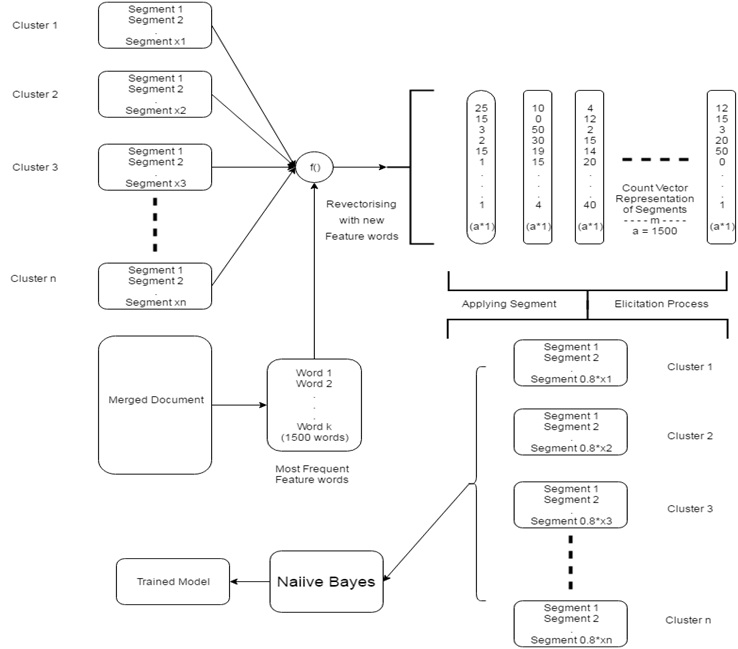
\includegraphics[width=8cm]{u6.jpg}
\centering
\end{figure}

\section{Data Set}
The data sets we have used to evaluate our model is:
\begin{itemize}
\item 690 blogs written by Gary Becker and Richard Posner.
\item	1,182 New York Times articles written by Maureen Dowd, Gail Collins, Thomas Freidman and Paul Krugman.\\
Each data set has its own set of challenges, since each author has written a lot of different topics and some topics are taken by both authors.
\end{itemize}
The resulting table is shown below:
\begin {table}[h]
\caption {Table Title} \label{tab:title} 
\begin{center}
 \begin{tabular}{||c c c c||}
 \hline
 Dataset & Accuracy & sentences & Authors \\ [0.5ex] 
 \hline\hline
 Becker-Posner & 0.82 & 26922 & 2 \\ 
 \hline
 GC-TF-PK & 0.67 & 11984 & 3 \\
 \hline
 MD-TF-PK & 0.70 & 13422 & 3 \\
 \hline
 MD-GC-PK & 0.66 & 13448 & 3 \\
 \hline
 MD-GC-TF-PK & 0.61 & 15584 & 4 \\ [1ex] 
 \hline
\end{tabular}
\end{center}
\end{table}


\section{Limitations of the Baseline System}
We can see that no deep NLP features are used for the task. A bag of words model is a weak model to be able to discriminate between the authors. Also, the accuracy of the final stage of classification depends on the “chunk” (V) of sentences picked from the individual authors to form the merged document. Changing that parameter (V) from 200 to 50 reduces the final accuracy from 82\% to 49\%. Training on segments and testing on sentences is not such a good idea as the whole bottleneck for achieving high accuracy is the clustering algorithm.
\begin{figure}
\caption{•}
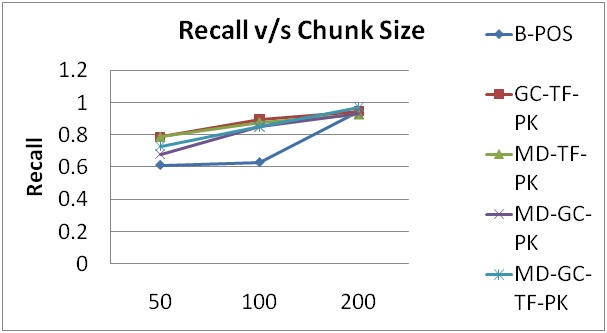
\includegraphics[width=8cm]{u4.jpg}
\centering
\end{figure}
\begin{figure}
\caption{•}
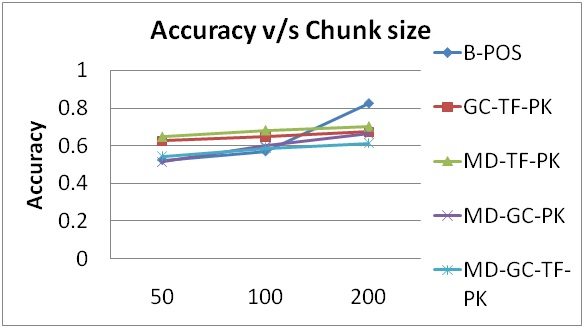
\includegraphics[width=8cm]{u5.jpg}
\centering
\end{figure}

\section{Proposed Methodology}
The main idea is to quantify the differences of the grammatical writing styles which the earlier baseline model was lacking and use this information to build paragraph clusters. So, by doing this, what kind of sentences can we decompose? An example shown below illustrates this. Consider the two sentences below:\\
\textit{S1: My chair started squeaking a few days ago and its driving me nuts.\\
S2: Since a few days my chair is squeaking-it’s simply annoying.\\}


The above sentences are semantically similar, although they differ way too much syntactically(as shown in the figure below) and a bag of words model, which just relies on the occurrences of the words/word counts can’t distinguish between these two sentences as they have more or less similar kinds of words. The main idea is to quantify those differences by calculating grammar profiles and to use this information to decompose a collaboratively written document.
\begin{figure}
\caption{•}
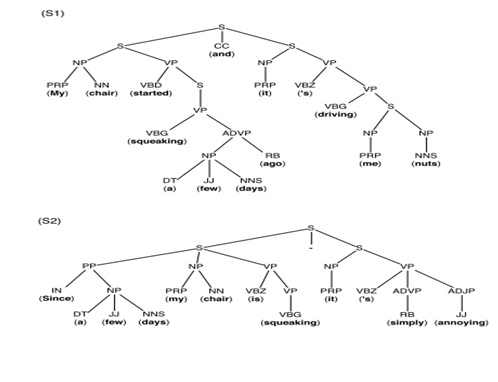
\includegraphics[width=8cm]{u2.jpg}
\end{figure}
\centering
\begin{figure}
\caption{The overview of our Method}
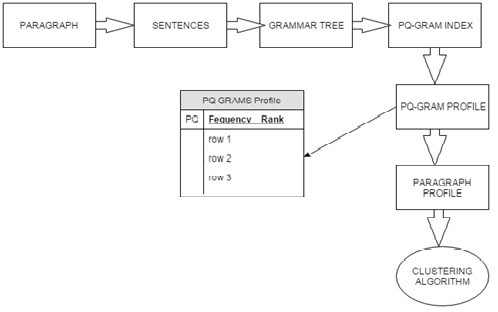
\includegraphics[width=8cm]{u3.jpg}
\centering
\end{figure}

\subsection{What is PQ Grams ?}
Similar to n-grams that represent the subparts of given length n of a string, p-q grams extract substructures of an ordered labelled tree. The size of p-q gram is determined by stem (p) and base (q). P defines how many nodes are included vertically, and q defines the number of nodes to be considered horizontally. For example, a valid p-q gram with p=2 and q=3 starting from PP at the left side of the tree (S2) shown in the above figure would be [PP-NP-DT-JJ-NNS ]. The p-q gram index then consists of all possible p-q grams of a tree. In order to obtain all p-q grams, the base is shifted left and right additionally. If less than p nodes exists horizontally, the corresponding place in the pq-gram is filled with \textbf{*}, indicating a missing node.\\

As seen from the flow chart above, paragraphs are extracted from text and each sentence is extracted from the paragraphs. For each sentences, a parse tree is formed using the standard StanfordParser. We call this the Grammar tree. From this Grammar tree, we extract the PQ Gram indices of these sentences. p-q gram index of a sentence is all possible p-q grams of a sentence , whereby multiple occurrences of the same p-q grams are also present multiple times in the index. By combining all p-q gram indices of all sentences, a p-q gram profile is created which contains a list of all p-q grams and their corresponding frequency of appearance in the text.
For our experiment, we have used p=2 and q=3. Finally, each paragraph-profile is provided as input for clustering algorithm, which are asked to build clusters based on the p-q grams contained. Also the labels are POS tags of Penn Treebank.


\subsection{Bottleneck}
When applied to the data set Becker-Posner dataset (26922 sentences), we encountered many long sentences which the parser was not able to parse.(out of memory). Below is a screenshot of the memory error we got. The sentence is 215 characters long.\\
One way out of this was to ignore all such sentences and proceed on the remaining “smaller” sentences, but that would have defeated the purpose of the baseline method, on whose results we were trying to improve upon.
Our observation from the above experiment is that, intuitively its a good method to capture the different syntactic aspects of writers. Although, it pushes the dimensionality of the feature space to quite high compared to the baseline. For 1000 sentences, we were getting a pq-gram profile size of 9200( and a training time of 120minutes), which will be quite high when run for more sentences. The baseline method’s feature size were much smaller and simpler and faster.

\begin{figure}
\caption{•}
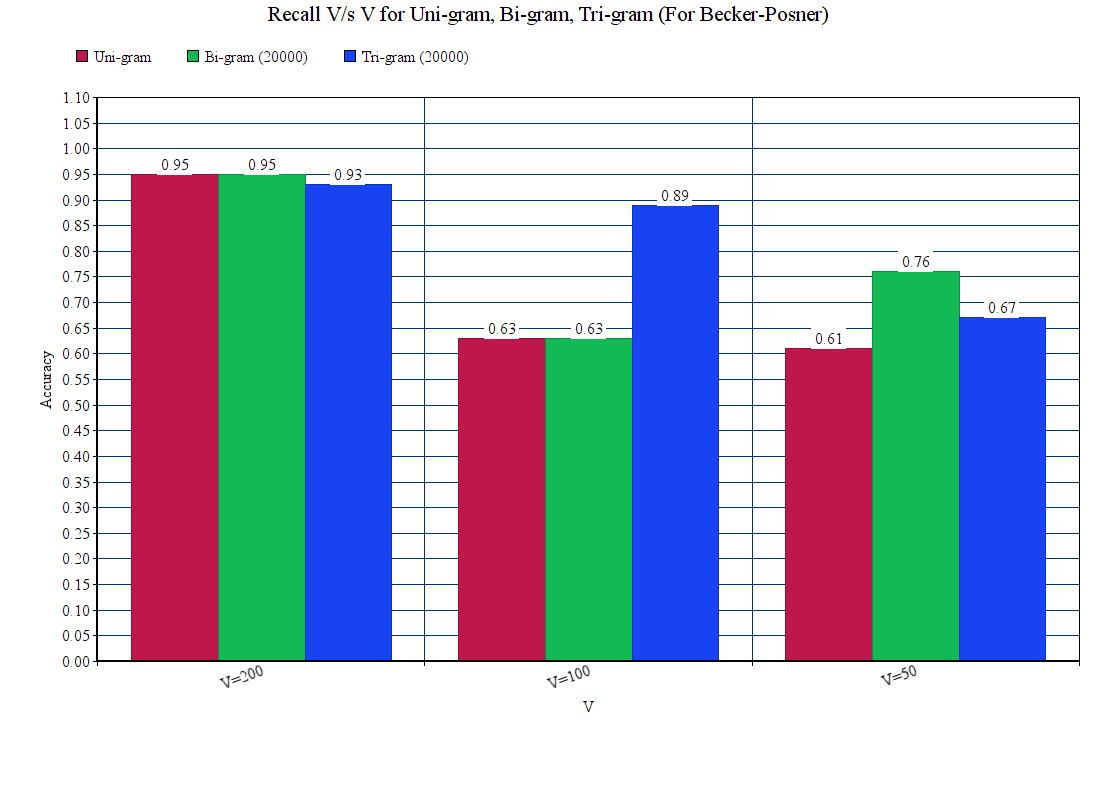
\includegraphics[width=8cm]{1.png}
\end{figure}
\begin{figure}
\caption{•}
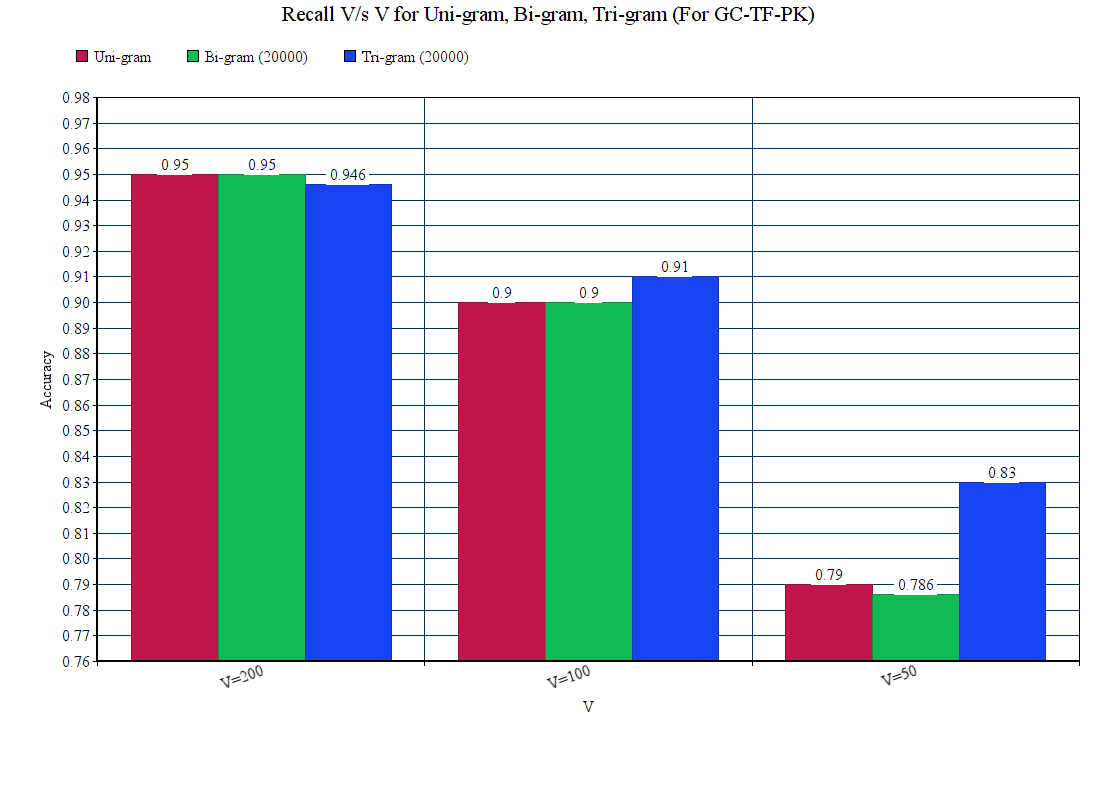
\includegraphics[width=8cm]{2.png}
\end{figure}
\begin{figure}
\caption{•}
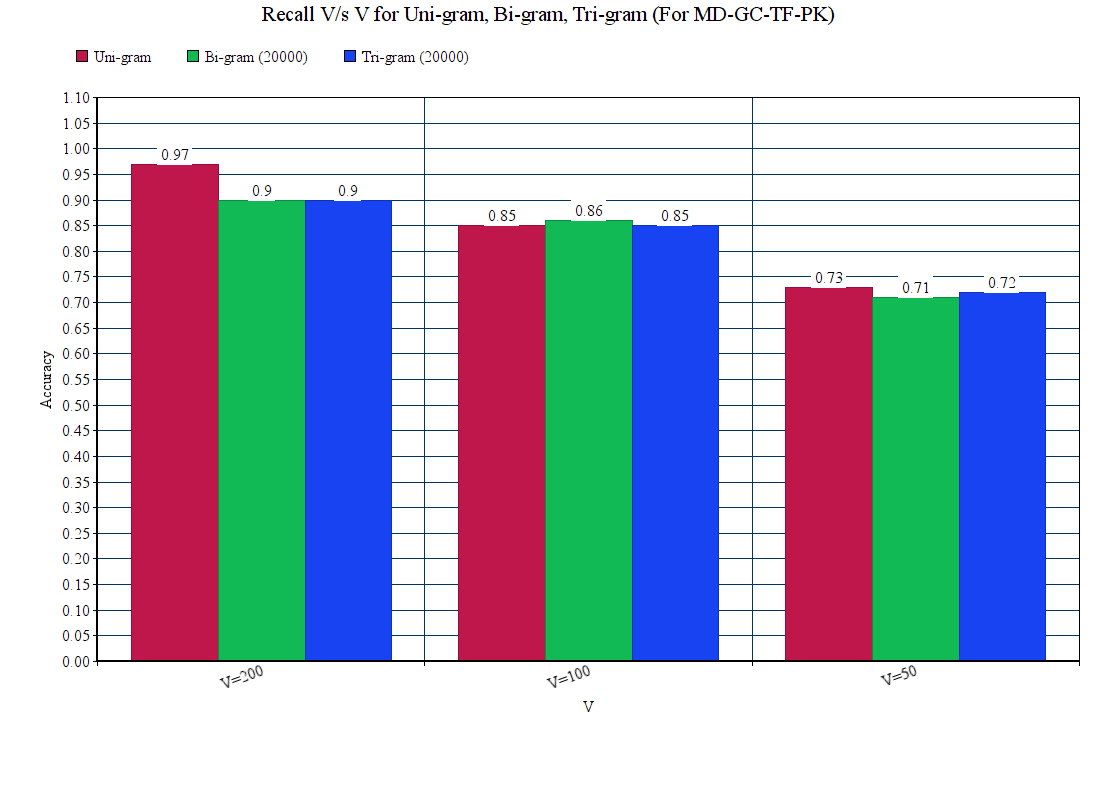
\includegraphics[width=8cm]{3.png}
\end{figure}
\begin{figure}
\caption{•}
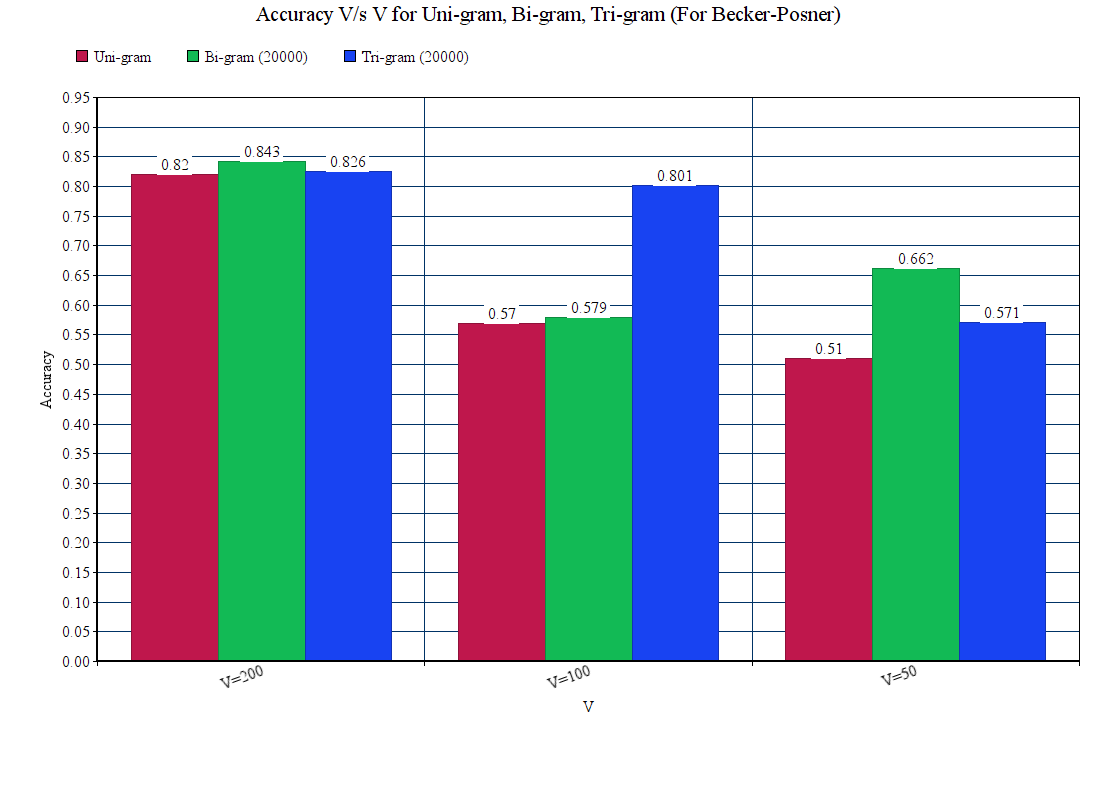
\includegraphics[width=8cm]{4.png}
\end{figure}
\begin{figure}
\caption{•}
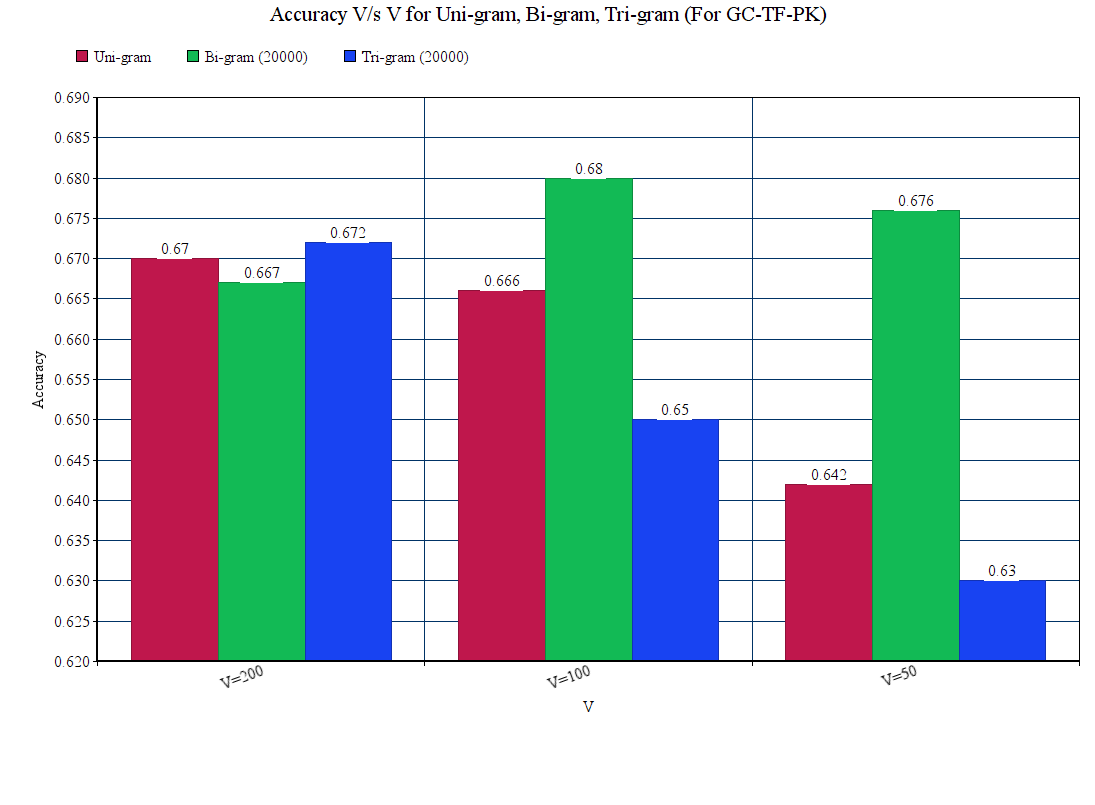
\includegraphics[width=8cm]{5.png}
\end{figure}
\begin{figure}
\caption{•}
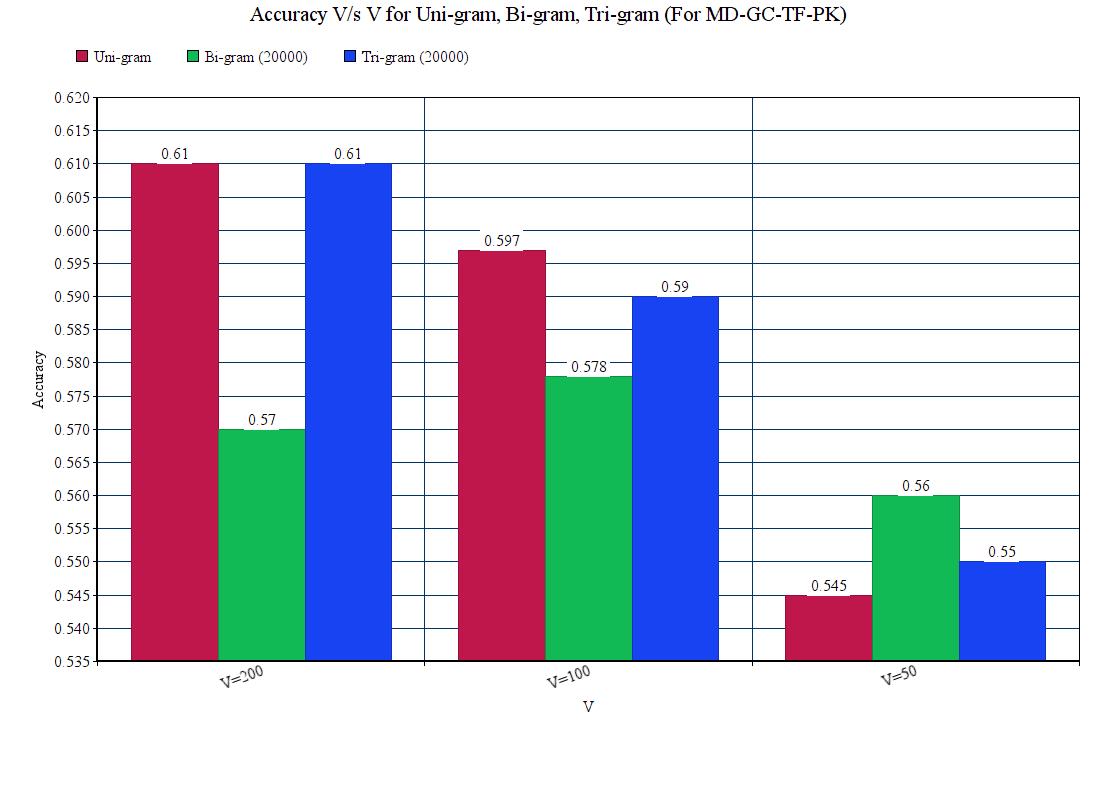
\includegraphics[width=8cm]{6.png}
\end{figure}

\subsection{References} 
\textit{A generic unsupervised method for decomposing multi-author documents.} Navot Akiva and Moshe Koppel.2013. \textit{Journal of the American Society for information Science and Technology,} 64: 2256--2264.
Navot Akiva and Moshe Koppel.2013. \textit{Science} 208: 1019--1026.\\
\textit{Unsupervised Decomposition of a Multi-Author Document Based on Naive-Bayesian Model.}Khaled Aldebei, Xiangjian He and Jie Yang. \textit{Proceedings of the 53rd Annual Meeting of the Association for Computational Linguistics (Short Papers)}, pages 501–505, Beijing, China

\end{document}